\chapter{Aprendizaje supervisado}
\label{chapter:super}
En este capítulo realizaremos el análisis de diferentes modelos supervisados que hemos construido con el fin de clasificar las llamadas en función de las etiquetas que hemos analizado en el capítulo \ref{chapter:dataset}.

Durante este capítulo describiremos las diferentes arquitecturas que proponemos para construir nuestros modelos (sección  \ref{section:super:arq}), posteriormente en la sección \ref{section:super:opt} evaluaremos la precisión de los modelos construidos con cada una de las arquitecturas propuestas y por último, en la sección \ref{section:super:mvm}, propondremos el modelo que pasaremos a producción y que hará de enlace con la siguiente parte del documento. 



\section{Arquitecturas}
\label{section:super:arq}

A lo largo de esta sección vamos a describir las diferentes arquitecturas que hemos utilizado para construir los modelos que posteriormente hemos entrenado y evaluado con los datos descritos en el capítulo anterior. 

\subsection{Red neuronal convolucional}

La primera aproximación a la hora de crear un modelo que nos permitiera clasificar llamadas, ha sido recurrir a las redes neuronales recurrente (que ya introdujimos en el estado del arte, en el apartado \ref{section:arte:arqu:cnn}). 

El objetivo que principal que perseguimos al aplicar esta estructura era poder capturar la estructura local de las llamadas, de una forma similar al modo en el que se hace en el tratamiento de imágenes. Aplicar \textit{kernels} de diferentes tamaños a la imagen inicial podía servirnos para obtener de manera automática especies de N-Gramas  que capten patrones en las transcripciones de las llamadas. 

\begin{figure}[!ht]
	\centering
	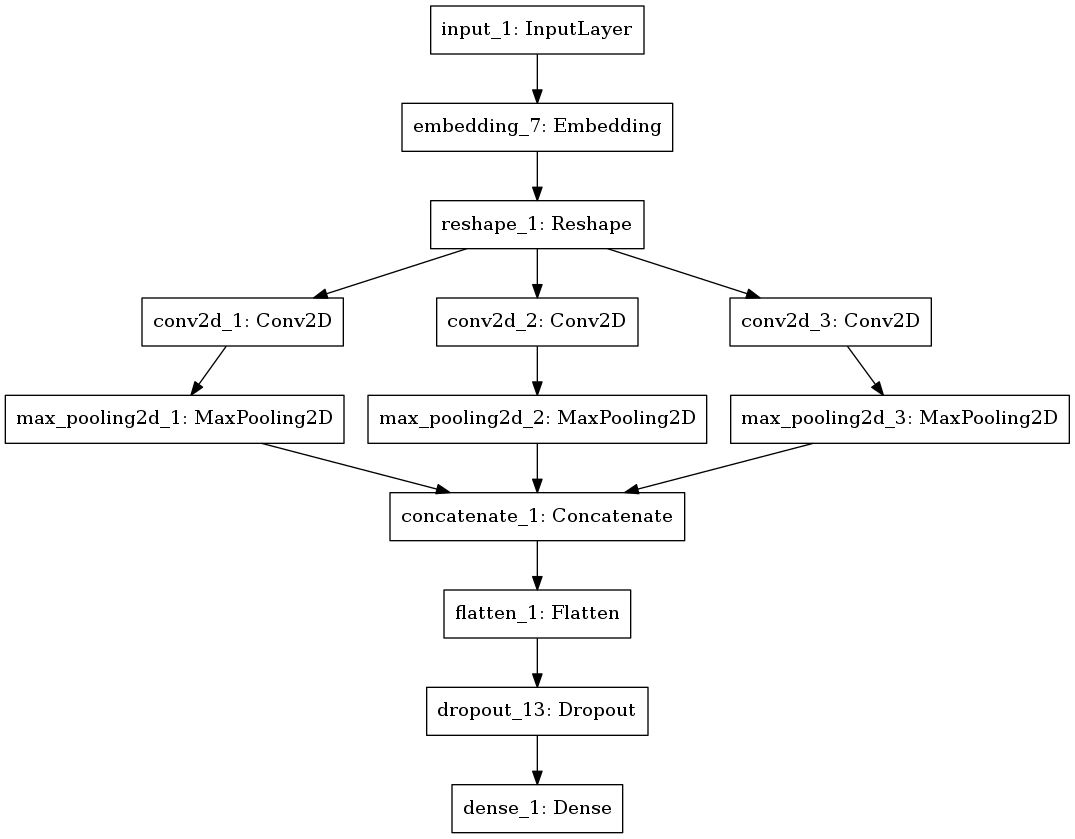
\includegraphics[width=0.7\textwidth]{images/super/arq_cnn}
	\caption{Arquitectura CNN}
	\label{fig:arqcnn}
\end{figure}


En la figura \ref{fig:arqcnn} podemos ver un ejemplo de un modelo de arquitectura de este tipo. Los modelos con la arquitectura que proponemos estarán formados por los siguientes tipos de capas: 

\begin{itemize}
\item \textbf{Entrada}: La entrada del modelo consistirá en una secuencia de identificadores de \textit{tokens}.

 \item \textbf{\textit{Embeddings}}: Una vez tengamos la entrada se le aplicará un \textit{embedding}, en nuestro caso hemos realizado la mayoría de los modelos con \textit{Skip-gram}. Este modelo estará pre-entrenado y simplemente traducirá cada \textit{ID} de la secuencia de palabras en el vector de números reales a partir de la matriz entrenada con anterioridad. 
 
 \item \textbf{Capas convolucionales}: Este será el núcleo de este tipo de modelos y consistirán en un número $N$ de capas en las que se aplicarán distintos tipos de \textit{kernels} al conjunto de entrada.
 
 
 \item \textbf{Capas \textit{Pooling}}: Se aplicara \textit{max-pooling} a la salida de cada una de las capas convolucionales. El objetivo es quedarnos con las características más relevantes de cada ``cuadrante''.
 
 
 \item \textbf{Capa de \textit{Dropout}}: Tras concatenar y aplanar la salida introduciremos una capa de \textit{dropout} previa a la capa totalmente conectada. El objetivo de esta capa será evitar el sobreentrenamiento. 
 
   \item \textbf{Capa totalmente conectada}: Por último, una capa totalmente conectada nos dará la salida del modelo. En función de si nuestro objetivo es clasificación multiclase o binaria utilizaremos como salida la función \textit{softmax} o \textit{sigmoid} respectivamente.
 
 
 
\end{itemize}

Esta arquitectura podrá utilizarse para crear diferentes parámetros, en nuestro caso hemos jugado con los parámetros: 

\begin{itemize}
\item Número de capas Convolucionales 
\item Tamaño de los \textit{kernels} que se aplicaran en cada capa.
\item Número de \textit{kernels} que tendrá cada capa. 
\item Valor de \textit{dropout}.
\item Valor de regularización nivel dos. Este parámetro intentará reducir el sobreentrenamiento de la red, reduciendo los pesos altos. 
\end{itemize}



El código de creación y entrenamiento de un modelo de este tipo, usando el módulo \textit{mgmtfm} sería: 
\vspace{0.5cm}
   
   
    \begin{tcolorbox}[breakable, size=fbox, boxrule=1pt, pad at break*=1mm,colback=cellbackground, colframe=cellborder]
\begin{Verbatim}[commandchars=\\\{\}]
\PY{n}{models\PYZus{}steps} \PY{o}{=} \PY{n}{models}\PY{o}{.}\PY{n}{Models}\PY{p}{(}\PY{n}{n\PYZus{}classes}\PY{p}{,}\PY{n}{input\PYZus{}shape}\PY{p}{,}\PY{n}{embedding\PYZus{}dim}\PY{p}{,}
                             \PY{n}{vocabulary\PYZus{}size}\PY{p}{,}\PY{n}{embedding\PYZus{}matrix}\PY{p}{)}
\PY{n}{models\PYZus{}steps}\PY{o}{.}\PY{n}{model\PYZus{}cnn\PYZus{}1}\PY{p}{(}\PY{n}{n\PYZus{}classes}\PY{p}{,}\PY{n}{filter\PYZus{}sizes}\PY{o}{=}\PY{n}{filter\PYZus{}sizes}\PY{p}{,} \PY{n}{drop}\PY{o}{=}\PY{n}{dropout}\PY{p}{,} 
                              \PY{n}{num\PYZus{}filters}\PY{o}{=}\PY{n}{num\PYZus{}filters}\PY{p}{)}
\PY{n}{models\PYZus{}steps}\PY{o}{.}\PY{n}{compile\PYZus{}and\PYZus{}train}\PY{p}{(}\PY{n}{X\PYZus{}train}\PY{p}{,} \PY{n}{y\PYZus{}train}\PY{p}{,}\PY{n}{batch\PYZus{}size}\PY{o}{=}\PY{n}{batch}\PY{p}{,}
                              \PY{n}{epochs}\PY{o}{=}\PY{n}{epochs}\PY{p}{,} \PY{n}{lr}\PY{o}{=}\PY{n}{lr}\PY{p}{,}\PY{n}{decay}\PY{o}{=}\PY{n}{decay}\PY{p}{,} 
                              \PY{n}{validation\PYZus{}data}\PY{o}{=}\PY{p}{(}\PY{n}{X\PYZus{}test}\PY{p}{,} \PY{n}{y\PYZus{}test}\PY{p}{)}\PY{p}{,}
                              \PY{n}{loss}\PY{o}{=}\PY{n}{loss\PYZus{}function}\PY{p}{)} 
\end{Verbatim}
\end{tcolorbox}
   
   


\subsection{Red neuronal recurrente}
En este apartado vamos a crear una arquitectura basándonos en otro de los modelos que vimos al analizar el estado del arte, las redes neuronales recurrentes (apartado \ref{section:arte:arqu:cnn}). De nuevo usaremos los modelos entrenados con este tipo de arquitectura para clasificar llamadas.

Las redes recurrentes a simple vista pueden parecer la solución más intuitiva a la hora de abordar un problema de análisis/clasificación de textos con \textit{Deep Learning}. En este caso iremos pasando toda la secuencia de \textit{tokens}, proveniente de la transcripción de nuestras llamadas, y, en cada paso (o \textit{token}), la red irá olvidando características poco relevantes del mensaje y quedándose con las características importantes para su clasificación. Como podemos imaginar el entrenamiento de estas redes es un proceso más complejo y costoso computacionalmente que el de las redes convolucionales anteriormente vistas.




\begin{figure}[!ht]
	\centering
	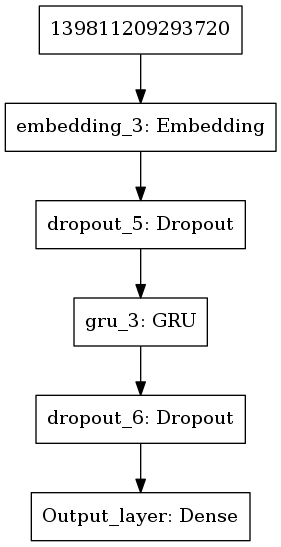
\includegraphics[width=0.25\textwidth]{images/super/arq_rnn1}
	\caption{Arquitectura RNN}
	\label{fig:arqrnn1}
\end{figure}


En la figura \ref{fig:arqrnn1} observamos un modelos de ejemplo con la arquitectura descrita. Los modelos con la arquitectura recurrente propuesta estarán formados por los siguientes tipos de capas: 

\begin{itemize}
\item \textbf{Entrada}: La entrada del modelo consistirá en una secuencia de identificadores de \textit{tokens}.

 \item \textbf{\textit{Embeddings}}: Una vez tengamos la entrada se le aplicará un \textit{embedding}, en nuestro caso hemos realizado la mayoría de los modelos con \textit{Skip-gram}. Este modelo estará pre-entrenado y simplemente traducirá cada \textit{ID} de la secuencia de palabras en el vector de números reales a partir de la matriz entrenada con anterioridad. 
 
 
  \item \textbf{Capa de \textit{Dropout}}:Posteriormente tendremos una capa de \textit{dropout} previa a la red recurrente. El objetivo de esta capa será evitar el sobreentrenamiento. Añadiremos otra capa de \textit{dropout} con el mismo objetivo previa a la capa totalmente conectada.
 
 \item \textbf{Capa recurrente}: En este punto introduciremos una capa formada por un número $N$ de celdas recurrentes. 
 
 
   \item \textbf{Capa totalmente conectada}: Por último, una capa totalmente conectada nos dará la salida del modelo. En función de si nuestro objetivo es clasificación multiclase o binaria utilizaremos como salida la función \textit{softmax} o \textit{sigmoid} respectivamente.
 
\end{itemize}


Esta arquitectura podrá utilizarse para crear diferentes modelos, en nuestro caso hemos jugado con los parámetros: 

\begin{itemize}
\item Tipo de celda: \textit{LSTM} o \textit{GRU}. 
\item Número de celdas en la capa recurrente. 
\item Valor de \textit{dropout}.
\end{itemize}


El código de creación y entrenamiento de un modelo de este tipo, usando el módulo \textit{mgmtfm} sería: 
\vspace{0.5cm}
   
    \begin{tcolorbox}[breakable, size=fbox, boxrule=1pt, pad at break*=1mm,colback=cellbackground, colframe=cellborder]
\begin{Verbatim}[commandchars=\\\{\}]
\PY{n}{models\PYZus{}steps} \PY{o}{=} \PY{n}{models}\PY{o}{.}\PY{n}{Models}\PY{p}{(}\PY{n}{n\PYZus{}classes}\PY{p}{,}\PY{n}{input\PYZus{}shape}\PY{p}{,}\PY{n}{embedding\PYZus{}dim}\PY{p}{,}
                               \PY{n}{vocabulary\PYZus{}size}\PY{p}{,}\PY{n}{embedding\PYZus{}matrix}\PY{p}{)}
\PY{n}{models\PYZus{}steps}\PY{o}{.}\PY{n}{model\PYZus{}rnn\PYZus{}1}\PY{p}{(}\PY{n}{memory\PYZus{}units}\PY{p}{,} \PY{n}{cell\PYZus{}type}\PY{p}{,} \PY{n}{dropout}\PY{p}{)}
\PY{n}{models\PYZus{}steps}\PY{o}{.}\PY{n}{compile\PYZus{}and\PYZus{}train}\PY{p}{(}\PY{n}{X\PYZus{}train}\PY{p}{,} \PY{n}{y\PYZus{}train}\PY{p}{,}
                                \PY{n}{batch\PYZus{}size}\PY{o}{=}\PY{n}{batch}\PY{p}{,} \PY{n}{epochs}\PY{o}{=}\PY{n}{epochs}\PY{p}{,} 
                                \PY{n}{lr}\PY{o}{=}\PY{n}{lr}\PY{p}{,}\PY{n}{decay}\PY{o}{=}\PY{n}{decay}\PY{p}{,}
                                \PY{n}{validation\PYZus{}data}\PY{o}{=}\PY{p}{(}\PY{n}{X\PYZus{}test}\PY{p}{,} \PY{n}{y\PYZus{}test}\PY{p}{)}\PY{p}{,}
                                \PY{n}{loss}\PY{o}{=}\PY{n}{loss\PYZus{}function}\PY{p}{)} 
\end{Verbatim}
\end{tcolorbox}


\subsection{Red neuronal ``híbrida'' convolucional/recurrente}

Vistas las características de ambas redes pensamos en combinar ambas para obtener las bondades de cada una. Por un lado una capa convolucional que se encargara de recoger las características locales de la secuencia (extraer los ``N-Gramas'') y posteriormente, una capa recurrente que utilice la información enriquecida por la capa convolucional para realizar la clasificación.



\begin{figure}[!ht]
	\centering
	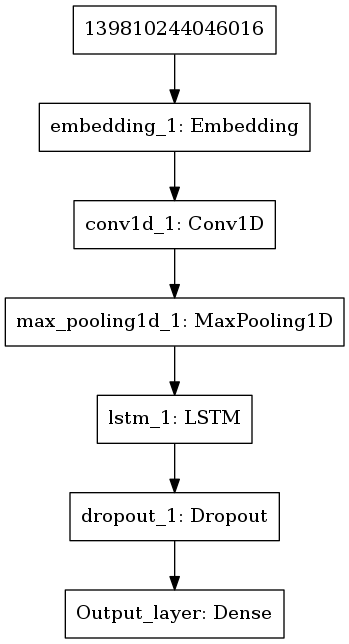
\includegraphics[width=0.25\textwidth]{images/super/arq_rnn2}
	\caption{Arquitectura ``Híbrida'' CNN/RNN}
	\label{fig:arqrnn2}
\end{figure}


En la figura \ref{fig:arqrnn2} podemos ver un ejemplo de un modelo de arquitectura de este tipo. Los modelos con la arquitectura que proponemos estarán formados por los siguientes tipos de capas:

 \begin{itemize}
 \item \textbf{Entrada}: La entrada del modelo consistirá en una secuencia de identificadores de \textit{tokens}.
 
  \item \textbf{\textit{Embeddings}}: Una vez tengamos la entrada se le aplicará un \textit{embedding}, en nuestro caso hemos realizado la mayoría de los modelos con \textit{Skip-gram}. Este modelo estará pre-entrenado y simplemente traducirá cada \textit{ID} de la secuencia de palabras en el vector de números reales a partir de la matriz entrenada con anterioridad. 
  
  \item \textbf{Capa convolucional}: En esta capa se aplicará un número determinado de \textit{kernels} con el tamaño especificado. 
  
 
  
  
  \item \textbf{Capas \textit{Pooling}}: Se aplicara \textit{max-pooling} a la salida de la capa convolucional. El objetivo es quedarnos con las características más relevantes de cada ``cuadrante''.
  
  
  \item \textbf{Capa de \textit{Dropout}}: Tras la capa recurrente introduciremos una capa de \textit{dropout} previa a la capa totalmente conectada. El objetivo de esta capa será evitar el sobreentrenamiento. 
  
  
   \item \textbf{Capa recurrente}: En este punto introduciremos una capa formada por un número $N$ de celdas recurrentes. 
   
  
    \item \textbf{Capa totalmente conectada}: Por último, una capa totalmente conectada nos dará la salida del modelo. En función de si nuestro objetivo es clasificación multiclase o binaria utilizaremos como salida la función \textit{softmax} o \textit{sigmoid} respectivamente.
  
  
 \end{itemize}


Esta arquitectura podrá utilizarse para crear diferentes modelos, en nuestro caso hemos jugado con los parámetros: 


\begin{itemize}

\item Tipo de celda de la capa recurrente: \textit{LSTM} o \textit{GRU}. 
\item Número de celdas en la capa recurrente. 
\item Valor de \textit{dropout}.
\item Tamaño de los \textit{kernels} que se aplicaran en la capa convolucional. 
\item Número de \textit{kernels} que tendrá la capa convolucional. 
\item \textit{padding} (str): Tipo de padding a realizar al aplicar la capa convolucional..
\end{itemize}

El código de creación y entrenamiento de un modelo de este tipo, usando el módulo \textit{mgmtfm} sería: 

\vspace{0.5cm}

    
    \begin{tcolorbox}[breakable, size=fbox, boxrule=1pt, pad at break*=1mm,colback=cellbackground, colframe=cellborder]

\begin{Verbatim}[commandchars=\\\{\}]
\PY{n}{models\PYZus{}steps} \PY{o}{=} \PY{n}{models}\PY{o}{.}\PY{n}{Models}\PY{p}{(}\PY{n}{n\PYZus{}classes}\PY{p}{,}\PY{n}{input\PYZus{}shape}\PY{p}{,}\PY{n}{embedding\PYZus{}dim}\PY{p}{,}
                               \PY{n}{vocabulary\PYZus{}size}\PY{p}{,}\PY{n}{embedding\PYZus{}matrix}\PY{p}{)}
\PY{n}{models\PYZus{}steps}\PY{o}{.}\PY{n}{model\PYZus{}rnn\PYZus{}2}\PY{p}{(}\PY{n}{memory\PYZus{}units}\PY{p}{,} \PY{n}{cell\PYZus{}type}\PY{p}{,} \PY{n}{dropout}\PY{p}{,}
                               \PY{n}{filters}\PY{p}{,}\PY{n}{filter\PYZus{}size}\PY{p}{,}\PY{n}{pooling\PYZus{}size}\PY{p}{,} \PY{n}{padding}\PY{p}{)}
\PY{n}{models\PYZus{}steps}\PY{o}{.}\PY{n}{compile\PYZus{}and\PYZus{}train}\PY{p}{(}\PY{n}{X\PYZus{}train}\PY{p}{,} \PY{n}{y\PYZus{}train}\PY{p}{,}\PY{n}{batch\PYZus{}size}\PY{o}{=}\PY{n}{batch}\PY{p}{,} 
                               \PY{n}{epochs}\PY{o}{=}\PY{n}{epochs}\PY{p}{,} \PY{n}{lr}\PY{o}{=}\PY{n}{lr}\PY{p}{,}\PY{n}{decay}\PY{o}{=}\PY{n}{decay}\PY{p}{,} 
                               \PY{n}{validation\PYZus{}data}\PY{o}{=}\PY{p}{(}\PY{n}{X\PYZus{}test}\PY{p}{,} \PY{n}{y\PYZus{}test}\PY{p}{)}\PY{p}{,}
                               \PY{n}{loss}\PY{o}{=}\PY{n}{loss\PYZus{}function}\PY{p}{)} 
\end{Verbatim}
\end{tcolorbox}






\subsection{MLP}
Los modelos que hemos visto hasta hora tenían siempre como entrada una secuencia de palabras, sin embargo con la representación de palabras \textit{Doc2Vec} es posible obtener un vector con números reales para cada transcripción que contenga información semántica del mismo. Esto nos permite poder abordar otro tipo de modelos más simples.  

\begin{figure}[!ht]
	\centering
	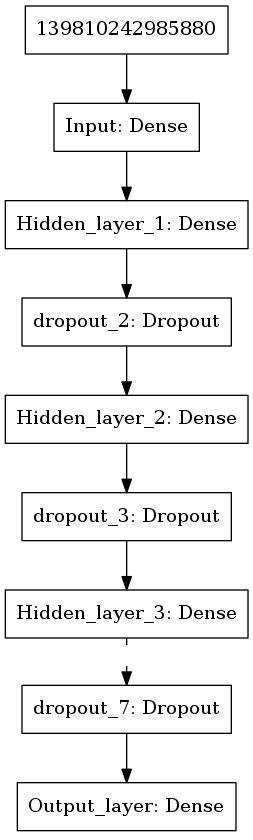
\includegraphics[width=0.20\textwidth]{images/super/arq_dense}
	\caption{Arquitectura con capas totalmente conectadas}
	\label{fig:arqdense}
\end{figure}

La arquitectura que proponemos, y que podemos ver en la figura \ref{fig:arqdense}, consiste en utilizar unicamente un número $N$ de capas totalmente conectadas y de \textit{dropout} (para evitar el sobreentrenamiento).

Los parámetros que podremos usar en este caso serían: 


\begin{itemize}

\item Número de capas totalmente conectadas. 
\item Número de neuronas en cada una de las capas. El número de neuronas de la última capa corresponderá con la salida y, en función de si nuestro objetivo es clasificación multiclase o binaria, utilizaremos como salida la función \textit{softmax} o \textit{sigmoid} respectivamente.
\item Valor de \textit{dropout}.
\end{itemize}


El código de creación y entrenamiento de un modelo de este tipo, usando el módulo \textit{mgmtfm} sería: 

\vspace{0.5cm}



    \begin{tcolorbox}[breakable, size=fbox, boxrule=1pt, pad at break*=1mm,colback=cellbackground, colframe=cellborder]
\begin{Verbatim}[commandchars=\\\{\}]
\PY{n}{models\PYZus{}steps} \PY{o}{=} \PY{n}{models}\PY{o}{.}\PY{n}{Models}\PY{p}{(}\PY{n}{n\PYZus{}classes}\PY{p}{,}\PY{n}{input\PYZus{}shape}\PY{p}{,}\PY{n}{embedding\PYZus{}dim}\PY{p}{,}
                               \PY{n}{vocabulary\PYZus{}size}\PY{p}{,}\PY{n}{embedding\PYZus{}matrix}\PY{p}{)}
\PY{n}{models\PYZus{}steps}\PY{o}{.}\PY{n}{model\PYZus{}dense\PYZus{}1}\PY{p}{(}\PY{n}{layers\PYZus{}list}\PY{p}{,}\PY{n}{drop}\PY{o}{=}\PY{n}{dropout}\PY{p}{)}
\PY{n}{models\PYZus{}steps}\PY{o}{.}\PY{n}{compile\PYZus{}and\PYZus{}train}\PY{p}{(}\PY{n}{X\PYZus{}train}\PY{p}{,} \PY{n}{y\PYZus{}train}\PY{p}{,}\PY{n}{batch\PYZus{}size}\PY{o}{=}\PY{n}{batch}\PY{p}{,} 
                               \PY{n}{epochs}\PY{o}{=}\PY{n}{epochs}\PY{p}{,} \PY{n}{lr}\PY{o}{=}\PY{n}{lr}\PY{p}{,}\PY{n}{decay}\PY{o}{=}\PY{n}{decay}\PY{p}{,} 
                               \PY{n}{validation\PYZus{}data}\PY{o}{=}\PY{p}{(}\PY{n}{X\PYZus{}test}\PY{p}{,} \PY{n}{y\PYZus{}test}\PY{p}{)}\PY{p}{,}
                               \PY{n}{loss}\PY{o}{=}\PY{n}{loss\PYZus{}function}\PY{p}{)} 
\end{Verbatim}
\end{tcolorbox}




\subsection{Combinación de modelos}
\label{section:super:mod:stack}

Otra opción que hemos abordado es la de combinar la salida de los modelos y que estos formen la entrada de un nuevo modelo de capas totalmente conectadas. 


\begin{figure}[!ht]
	\centering
	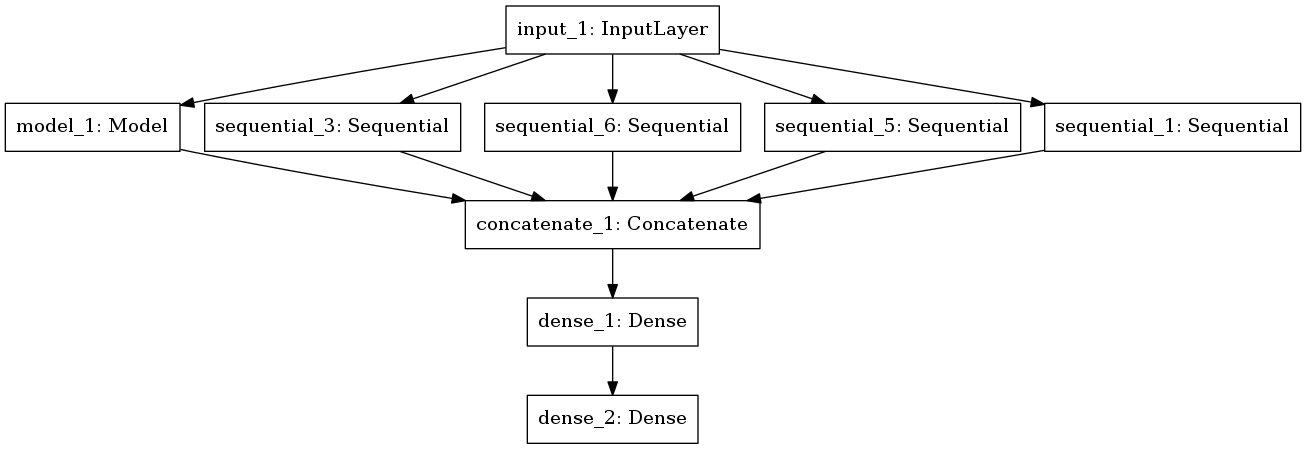
\includegraphics[width=1\textwidth]{images/super/arq_stack}
	\caption{Arquitectura con capas totalmente conectadas}
	\label{fig:arqstack}
\end{figure}


En la figura \ref{fig:arqstack}, vemos un ejemplo de este tipo de modelos. En este caso el input alimenta a los diferentes modelos (5 en este caso), que pueden estar construidos tanto con el modelo \textit{Model} de keras como con el modelo \textit{Sequential}.


La salida de los diferentes modelos se concatena y, antes de la salida, se añade una capa oculta totalmente conectada con función de activación \textit{relu}. Normalmente este tipo de modelos no vamos a usarlos en clasificación binaria por lo que la función de activación de la capa de salida será sigmoid.


Hay que destacar que los sub-modelos que forman parte de este modelo están preentrenados y no volverán a entrenarse en el proceso de aprendizaje.


En este caso no tenemos implementado el modelo en el módulo \textit{mgmtfm}, pero podemos basarnos en una lista de modelos creados en \textit{mgmtfm} ``$prev\_models$'' para crearlo: 
\vspace{0.5cm}

    \begin{tcolorbox}[breakable, size=fbox, boxrule=1pt, pad at break*=1mm,colback=cellbackground, colframe=cellborder]
\begin{Verbatim}[commandchars=\\\{\}]
\PY{k+kn}{from} \PY{n+nn}{keras}\PY{n+nn}{.}\PY{n+nn}{layers} \PY{k}{import} \PY{n}{Input}\PY{p}{,} \PY{n}{Dense}\PY{p}{,}  \PY{n}{concatenate}
\PY{k+kn}{from} \PY{n+nn}{keras}\PY{n+nn}{.}\PY{n+nn}{models} \PY{k}{import} \PY{n}{Model}

\PY{k}{for} \PY{n}{pm} \PY{o+ow}{in} \PY{n}{prev\PYZus{}models}\PY{p}{:}
    \PY{k}{for} \PY{n}{layer} \PY{o+ow}{in} \PY{n}{pm}\PY{o}{.}\PY{n}{\PYZus{}model}\PY{o}{.}\PY{n}{layers}\PY{p}{:}
        \PY{n}{layer}\PY{o}{.}\PY{n}{trainable} \PY{o}{=} \PY{k+kc}{False}


\PY{n}{models\PYZus{}out} \PY{o}{=} \PY{p}{[}\PY{n}{pm}\PY{o}{.}\PY{n}{\PYZus{}model}\PY{p}{(}\PY{n}{in\PYZus{}model}\PY{p}{)} \PY{k}{for} \PY{n}{pm} \PY{o+ow}{in} \PY{n}{prev\PYZus{}models}\PY{p}{]}
\PY{n}{combined} \PY{o}{=} \PY{n}{concatenate}\PY{p}{(}\PY{n}{models\PYZus{}out}\PY{p}{)}
\PY{n}{hidden} \PY{o}{=} \PY{n}{Dense}\PY{p}{(}\PY{n}{n\PYZus{}hidden}\PY{p}{,} \PY{n}{activation}\PY{o}{=}\PY{l+s+s1}{\PYZsq{}}\PY{l+s+s1}{relu}\PY{l+s+s1}{\PYZsq{}}\PY{p}{)}\PY{p}{(}\PY{n}{combined}\PY{p}{)}
\PY{n}{out\PYZus{}model} \PY{o}{=} \PY{n}{Dense}\PY{p}{(}\PY{n}{n\PYZus{}classes}\PY{p}{,} \PY{n}{activation}\PY{o}{=}\PY{l+s+s1}{\PYZsq{}}\PY{l+s+s1}{softmax}\PY{l+s+s1}{\PYZsq{}}\PY{p}{)}\PY{p}{(}\PY{n}{hidden}\PY{p}{)}
\PY{n}{model} \PY{o}{=} \PY{n}{Model}\PY{p}{(}\PY{n}{in\PYZus{}model} \PY{p}{,} \PY{n}{out\PYZus{}model}\PY{p}{)}
\end{Verbatim}
\end{tcolorbox}

Y posteriormente entrenarlo: 

\vspace{0.5cm}

    \begin{tcolorbox}[breakable, size=fbox, boxrule=1pt, pad at break*=1mm,colback=cellbackground, colframe=cellborder]
\begin{Verbatim}[commandchars=\\\{\}]
\PY{k+kn}{from} \PY{n+nn}{keras}\PY{n+nn}{.}\PY{n+nn}{optimizers} \PY{k}{import} \PY{n}{Adam}
\PY{k+kn}{from} \PY{n+nn}{keras}\PY{n+nn}{.}\PY{n+nn}{preprocessing}\PY{n+nn}{.}\PY{n+nn}{sequence} \PY{k}{import} \PY{n}{pad\PYZus{}sequences}

\PY{n}{adam} \PY{o}{=} \PY{n}{Adam}\PY{p}{(}\PY{n}{lr}\PY{p}{,} \PY{n}{decay}\PY{o}{=}\PY{n}{decay}\PY{p}{)}
        
\PY{n}{model}\PY{o}{.}\PY{n}{compile}\PY{p}{(}\PY{n}{loss}\PY{o}{=}\PY{n}{loss}\PY{p}{,}
                    \PY{n}{optimizer}\PY{o}{=}\PY{n}{adam}\PY{p}{,}
                    \PY{n}{metrics}\PY{o}{=}\PY{n}{metrics}  \PY{p}{)}

\PY{n}{model}\PY{o}{.}\PY{n}{fit}\PY{p}{(}\PY{n}{X\PYZus{}train}\PY{p}{,} \PY{n}{y\PYZus{}train}\PY{p}{,} \PY{n}{batch\PYZus{}size}\PY{o}{=}\PY{n}{batch\_size}\PY{p}{,} \PY{n}{epochs}\PY{o}{=}\PY{n}{epochs}\PY{p}{,}
                        \PY{n}{validation\PYZus{}data}\PY{o}{=}\PY{p}{(}\PY{n}{X\PYZus{}test} \PY{p}{,} \PY{n}{y\PYZus{}test}\PY{p}{)}\PY{p}{)} 
\end{Verbatim}
\end{tcolorbox}



\section{Evaluación y optimización}
\label{section:super:opt}
Una vez hemos creados los modelos acordes a las diferentes arquitecturas comentadas en el apartado anterior surge la necesidad de encontrar los hiperparámetros que en cada arquitectura nos lleven a la mayor precisión de nuestro modelo.


Encontrar los mejores parámetros es una tarea crucial a la hora de probar un modelo y ,aunque existen diferentes métodos para intentar conseguir los mejores resultados al entrenar nuestro modelo, como puede ser definir un \textit{Grid} de parámetros o probar de manera aleatoria; nosotros hemos probado por un mecanismo más automático utilizando \textit{\textbf{Optuna}}.

\textit{Optuna} es un \textit{framework} de optimización de modelos que utiliza métodos Bayesianos para la optimización de modelos.  Entre las ventajas de \textit{Optuna} tenemos: 

\begin{itemize}
\item Utilización de una BBDD (en nuestro caso \textit{PostgreSQL}) que nos permite continuar con los entrenamientos cuando queramos y lanzar varios entrenamientos en paralelo o en cualquier momento. 
\item Posibilidad de definir la duración de las pruebas que queremos lanzar. Lo que nos permite, por ejemplo, lanzar pruebas por la noche cuando el cluster posee más recursos.  

\item Uso de la poda para descartar modelos con mala calidad en fases tempranas, ahorrando tiempo de cómputo. 
\end{itemize}


Desde que empezamos a usar \textit{Optuna} en la plataforma formada por \textit{GPUs} $Tesla V100-SXM2 32GB$, hemos dedicado unas 340 horas a la optimización de modelos, lo que supone algo más de 14 días. Hay que tener en cuenta que muchas de las pruebas no prometedoras \textit{Optuna} las ha cancelado automáticamente, por lo que en condiciones normales hubiéramos necesitado bastante más tiempo. También hay momentos en los que se ha paralelizado el entrenamiento entre varias \textit{GPUs}.


A lo largo del apartado veremos las distintas pruebas realizadas agrupándolas por tipo de arquitectura. Los nombres de los modelos nos darán
información sobre el tipo del modelo. Algunos datos que tenemos que
tener en cuenta son:
\begin{itemize}
 

\item \textbf{\textit{CNN/RNN/RNN2/DENSE}}: Nos indica el tipo del modelo y estará al comienzo
del nombre.

\item \textbf{\textit{IVR/MONI}}: Nos indica si el modelo ha sido entrenado y validado con los
tipos de IVR o de monitorizaciones. De momento solo usamos \textit{IVR} debido a la poca cantidad de transcripciones que tenemos con datos de monitorizaciones..

\item \textbf{\textit{W2V150QC}}: Nos indica que utiliza un \textit{Word2Vec} con una dimensión de 150 y
quitando las palabras comunes en los \textit{tokens}.

\item \textbf{\textit{BIN/MULTI}}: Nos indica que se trata de un modelo binario o multiclase. Si
es binario al final del nombre nos encontramos la clase, si es multiclase y
no clasifica todas las clases nos encontramos las iniciales de las
clases.

\item \textbf{\textit{QX}}: Nos indica las clases que se eliminan. Por ejemplo \textit{QR\_QN} elimina
las clases resto y no reconocido antes de entrenar. La no reconocido la
eliminamos siempre ya que puede contener varias clases.

\item \textbf{\textit{866}}: Indica que en estos modelos se ha limitado las secuencias a 866
tokens, que engloban más del 99\% de las llamadas.

 \end{itemize}

Una última consideración a tener en cuenta es que, solo los modelos más prometedores se han pasado a la fase de optimización con \textit{Optuna}. Otros tantos, como pueden ser los modelos con datos de monitorizaciones, se han descartado desde un primer momento observando que los primeros resultados no eran prometedores.

\subsection{Modelos \textit{CNN} binarios}
Aunque se han hecho pruebas con modelos multi-clase, cuando se ha
empezado a utilizar \textit{Optuna} unicamente se han entrenado modelos binarios
que presentaban mucho mejores resultados. Por ello en esta primera sesión únicamente presentaremos datos de modelos convolucionales. 

Para cada modelo mostraremos los siguientes campos: 

\begin{itemize}
\item \textbf{\textit{study}}: Nombre del modelo del que se está realizando el estudio. 
\item \textbf{\textit{accuracy}}: Mejor precisión sobre el conjunto de test.
 \item \textbf{\textit{params}}: Parámetros con los que se ha obtenido la mejor precisión. 
  \item \textbf{\textit{ntrials}}: Número de pruebas realizadas del estudio. Cuenta las pruebas podadas, pero no las fallidas. 
    \item \textbf{\textit{total\_time}}: Tiempo total invertido en el entrenamiento del modelo.
    \item \textbf{\textit{best\_trial}}: Identificador de la mejor prueba realizada. Nos será de utilidad ya que \textit{Optuna} guarda los pesos automáticamente del mejor modelo.
\end{itemize}


\begin{figure}[!ht]
	\centering
	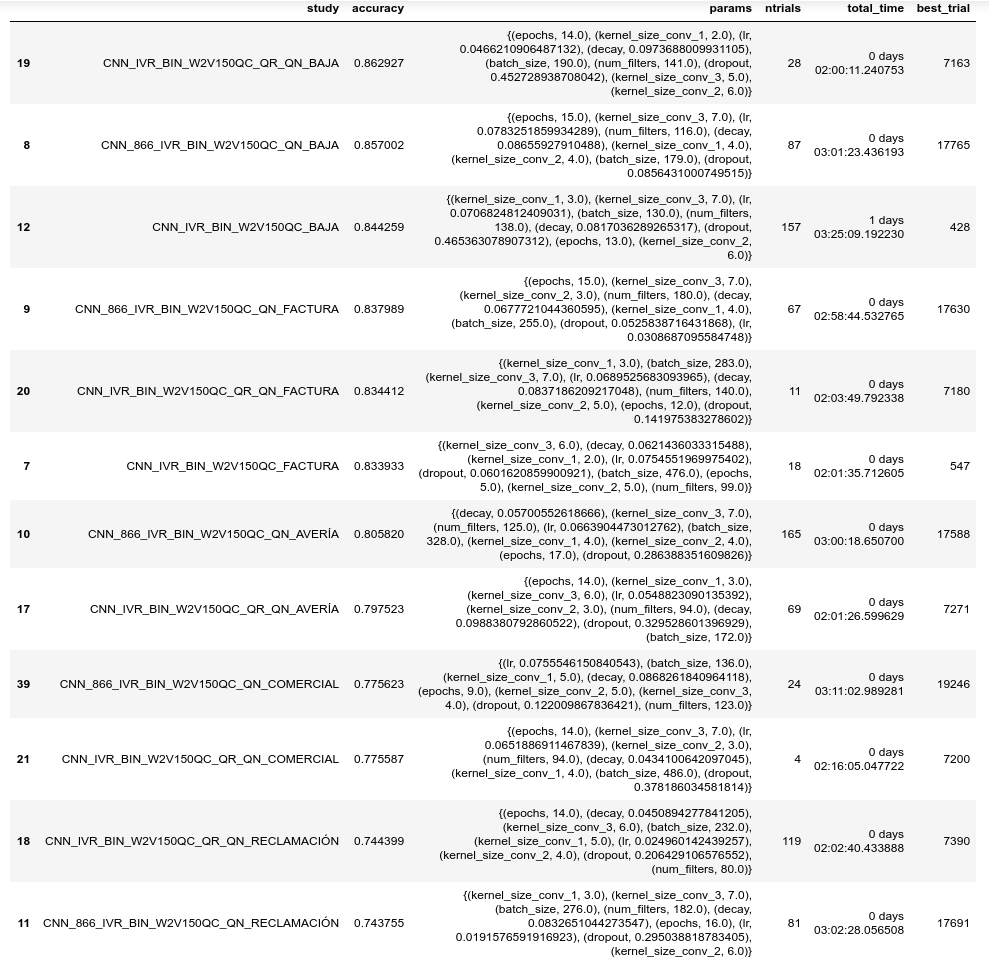
\includegraphics[width=1\textwidth]{images/super/opt_cnn}
	\caption{Optimización de modelos binarios con redes convolucionales}
	\label{fig:opt_cnn}
\end{figure}

  Los modelos se han entrenado
 con datos balanceados, teniendo el mismo número de muestras de la clase binaria y del resto de
clases. 


En la figura \ref{fig:opt_cnn} podemos ver los resultados obtenidos. Los resultados parecen bastante buenos para la mayoría de clases que van desde el 72\% al 86\% de precisión. Cuando eliminamos las clases resto y no reconocido vemos que los datos mejoran. Esto se debe a que, probablemente, existan datos 


\subsection{Modelos \textit{RNN} Binarios}

A continuación presentamos los resultados de los modelos formados por redes recurrentes que realizan clasificación binaria en el mismo formato que el apartado anterior. Hemos agrupado en los modelos recurrentes también aquellos que tienen una capa convolucional junto a la capa recurrente. 

\begin{figure}[!ht]
	\centering
	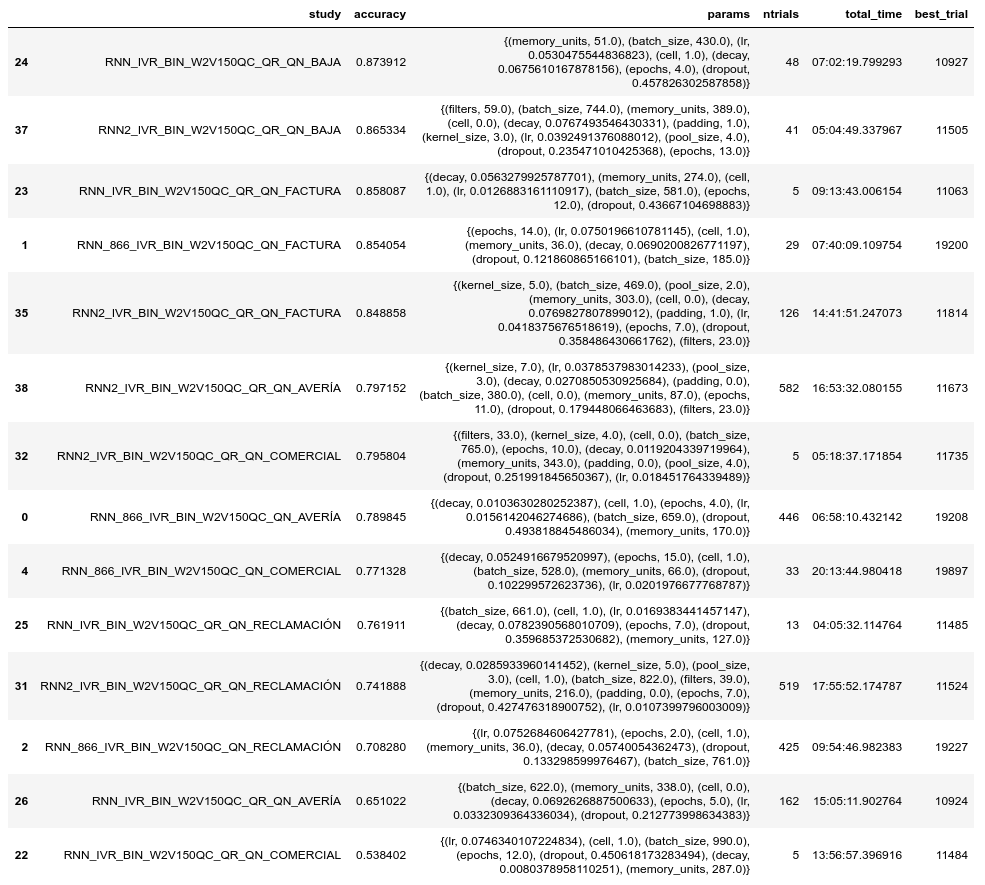
\includegraphics[width=1\textwidth]{images/super/opt_rnn_bin}
	\caption{Optimización de modelos binarios con redes recurrentes}
	\label{fig:opt_rnn}
\end{figure}


En general, observando la figura \ref{fig:opt_rnn}, vemos una ligera mejora con respecto a los modelos formados por redes convolucionales. Vemos por ejemplo como en el caso de la clase \textit{Factura} hemos mejorado el modelo hasta casi el 86\% con una red recurrente y el caso de la clase \textit{Comercial} con una red recurrente con una capa convolucional hemos llegado al 79.6\%. 

También podemos observar que no existe una diferencia apreciable entre los modelos que incluyen una capa convolucional y los que no la tienen. Otro punto a destacar de estas pruebas es que el tiempo de ejecución medio, si observamos el tiempo total y el número de pruebas, es mucho mayor que en los modelos convolucionales. 

En cuanto al tipo de celdas vemos que aunque aparecen ambos (valor 0 para $LSTM$ y valor 1 para $GRU$) los mejores resultados los hemos obtenido con $GRU$ siendo además los modelos con este tipo de celdas menos costosos para el entrenamiento. 

\subsection{Modelos totalmente conectados}

A continuación presentamos algunas pruebas, también de clasificación binaria, que realizamos utilizando como entrada directamente los vectores \textit{Doc2Vec} de las transcripciones.  

\begin{figure}[!ht]
	\centering
	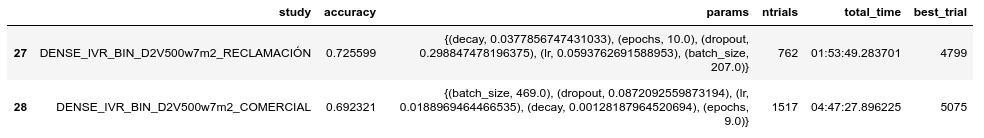
\includegraphics[width=1\textwidth]{images/super/opt_dense}
	\caption{Optimización de modelos binarios con \textit{MLP}}
	\label{fig:opt_dense}
\end{figure}

Como observamos en la figura \ref{fig:opt_dense}, unicamente hemos realizado pruebas de optimización con las clases \textit{Reclamación} y \textit{Comercial} devolviendo unos resultados de precisión sobre el conjunto de test del 72\% y 69\% respectivamente. El hecho de que los modelos anteriormente presentados tuvieran una mayor precisión nos llevó a no continuar por esta vía. 
 

\subsection{Modelos multiclase}

Hasta ahora todos los modelos que hemos presentado son binarios y hemos tenido resultados bastante aceptables en estos casos. En este apartado vamos a mostrar modelos multiclase basados en las mismas arquitecturas vistas anteriormente.



\begin{figure}[!ht]
	\centering
	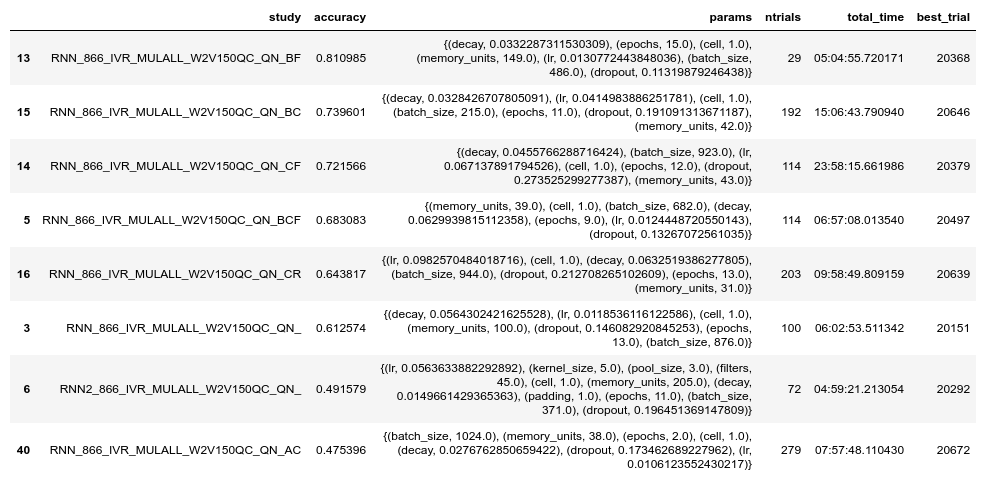
\includegraphics[width=1\textwidth]{images/super/opt_multi}
	\caption{Optimización de modelos multiclase}
	\label{fig:opt_multi}
\end{figure}

En la figura \ref{fig:opt_multi}  los modelos multiclase que hemos construido y optimizado. Vemos que todos ellos los hemos construido con redes recurrentes de distintos tipos, que son las que, hasta ahora, nos han dado mejores resultados.  Aunque hicimos también  varias pruebas de conectar varios modelos binarios con la arquitectura propuesta en \ref{section:super:mod:stack} los resultados no fueron satisfactorio y la calidad disminuía considerablemente. 


Las últimas iniciales del campo \textit{study} nos indican las clases que el modelo es capaz de distinguir, si acaba en ``\_'' el modelo clasifica entre todas las clases.

Vemos que la mejor precisión en un modelo multiclase la tenemos hasta el momento en un modelo con redes recurrentes que distingue entre Bajas, Facturas y el resto de llamadas con una precisión del 81\%.


\section{Modelo Mínimo Viable}
\label{section:super:mvm}
El título de este apartado esta basado en el concepto de mínimo producto viable (MVP por sus siglas en inglés) acuñado por la metodología \textit{Lean Startup}. Un producto mínimo viable debe reunir las características mínimas para satisfacer a los primeros clientes y poder crear una retroalimentación que ayude a que sea mejorado en el futuro. En nuestro caso queremos llevar a producción uno de los modelos diseñados hasta ahora para poder construir un sistema completo y obtener \textit{feedack} que nos ayude en futuras mejoras.

El modelo que hemos seleccionado es el mejor modelo del estudio ``RNN\_866\_IVR\_MULALL\_W2V150QC\_QN\_BF'' y podemos verlo en la figura \ref{fig:opt_multi}. Se trata de un modelo basado en la arquitectura de redes recurrentes, con 149 celdas tipo $GRU$ y que toma como entrada una secuencia de 866 \textit{Tokens} (El 99\% de las transcripciones están por debajo de este número de \textit{tokens}).

A continuación vamos a volver a medir la precisión del modelo usando tanto datos balanceados como sin balancear con el objetivo de verificar que el modelo pueda ser usado en un entorno productivo.


\begin{figure}[!ht]
	\centering
	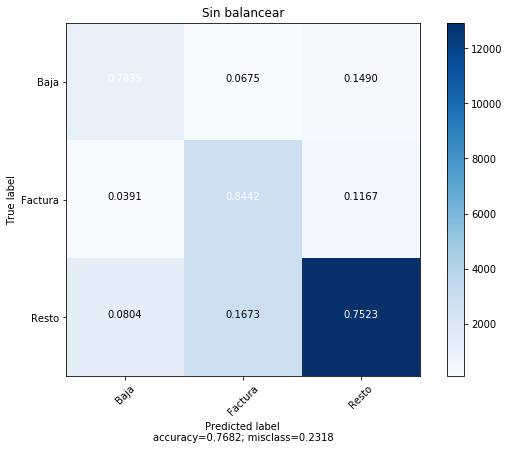
\includegraphics[width=0.6\textwidth]{images/super/mvp_mat1}
	\caption{Matriz de confusión datos balanceados}
	\label{fig:mvp_mat1}
\end{figure}


\begin{figure}[!ht]
	\centering
	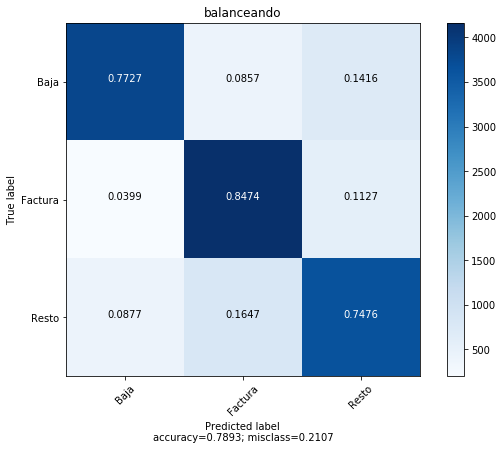
\includegraphics[width=0.6\textwidth]{images/super/mvp_mat2}
	\caption{Matriz de confusión datos no balanceados}
	\label{fig:mvp_mat2}
\end{figure}

En la figura \ref{fig:mvp_mat1} podemos ver la precisión del modelo con datos balanceados, mientras que en la figura  \ref{fig:mvp_mat2} vemos estos mismos datos sin balancear. Observamos que en el modelo sin balancear la mayoría de muestras se concentran en el resto, lo que es normal, ya que hay más llamadas de otros tipos que de \textit{Baja} y \textit{Factura}. Sin embargo, podemos ver que la precisión no varía sustancialmente por lo que el modelo es suceptible de usar en producción.


La siguiente parte del documento tratará de llevar a producción este modelo para que sea capaz de clasificar las llamadas en tiempo real con todo lo que ello implica. A partir de ahora nos referiremos a el como el modelo \textit{\textbf{bajafactura}} y lo veremos como una caja negra en la que solo nos preocuparemos por la forma en la que debemos introducir los datos y por las clasificaciones devueltas por el mismo.

